% This file was created with matplot2tikz v0.5.4.
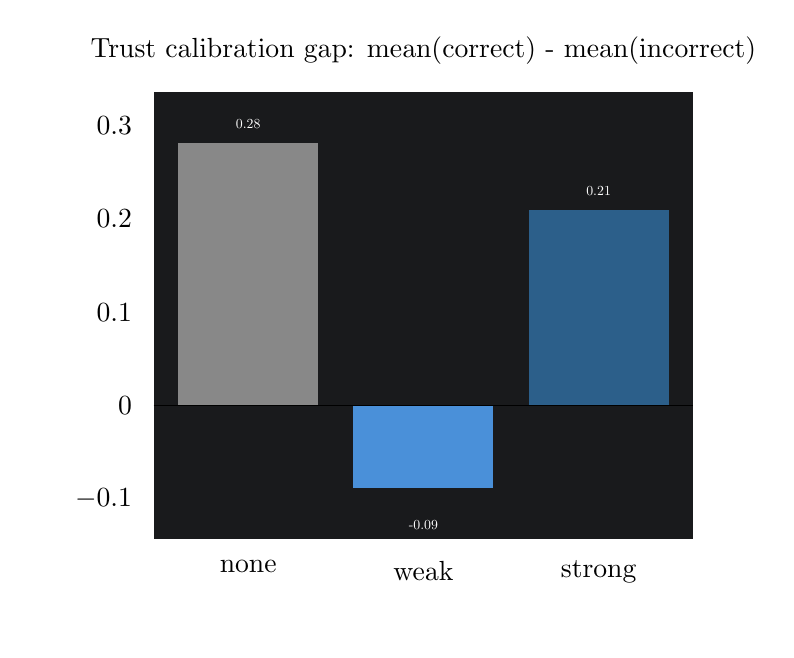
\begin{tikzpicture}

\definecolor{black252628}{RGB}{25,26,28}
\definecolor{cornflowerblue74144217}{RGB}{74,144,217}
\definecolor{darkgray176}{RGB}{176,176,176}
\definecolor{darkslateblue4495138}{RGB}{44,95,138}
\definecolor{gray136}{RGB}{136,136,136}

\begin{axis}[
axis background/.style={fill=black252628},
axis line style={white},
tick align=outside,
tick pos=left,
title={Trust calibration gap: mean(correct) - mean(incorrect)},
x grid style={darkgray176},
xlabel=\textcolor{white}{attestation},
xmin=-0.54, xmax=2.54,
xtick style={color=white},
xtick={0,1,2},
xticklabels={none,weak,strong},
y grid style={darkgray176},
ylabel=\textcolor{white}{trust difference},
ymin=-0.143205871465589, ymax=0.33701985629811,
ytick style={color=white}
]
\draw[draw=none,fill=gray136] (axis cs:-0.4,0) rectangle (axis cs:0.4,0.281609195402299);
\draw[draw=none,fill=cornflowerblue74144217] (axis cs:0.6,0) rectangle (axis cs:1.4,-0.0877952105697775);
\draw[draw=none,fill=darkslateblue4495138] (axis cs:1.6,0) rectangle (axis cs:2.4,0.209302325581395);
\addplot [line width=0.32pt, black]
table {%
-0.54 0
2.54 0
};
\draw (axis cs:0,0.291609195402299) node[
  scale=0.5,
  anchor=south,
  text=white,
  rotate=0.0
]{0.28};
\draw (axis cs:1,-0.117795210569777) node[
  scale=0.5,
  anchor=north,
  text=white,
  rotate=0.0
]{-0.09};
\draw (axis cs:2,0.219302325581395) node[
  scale=0.5,
  anchor=south,
  text=white,
  rotate=0.0
]{0.21};
\end{axis}

\end{tikzpicture}
